\documentclass[12pt]{article}
\usepackage[utf8]{inputenc}
\usepackage[margin=0.8in]{geometry}

    % Related to mæth :)
\usepackage{amsmath,amssymb,amsfonts,amsthm}
%\usepackage{scrlayer-scrlayer}
\usepackage{scrlayer-scrpage}
\usepackage{tikz}
\usepackage{multicol}
\usepackage{algorithm}
\usepackage{algpseudocode}
\usepackage{listings}
\usepackage{xcolor}
\usepackage{color}
\usepackage{textcomp}

\usepackage{enumerate}
\pagestyle{scrheadings}

\title{Aufgabe 4\\Streichholzrätsel}
\author{Tassilo Tanneberger}
\newcommand{\linia}{\rule{\linewidth}{1pt}}
\makeatletter
\renewcommand{\maketitle}{
\begin{center}
\huge \@title
\end{center}
\linia\\
{\large\@author\hfill 3.11.2020\\}}

%==========================================================

\graphicspath{ {./resources/} }

%==========================================================

\definecolor{codegreen}{rgb}{0,0.6,0}
\definecolor{codegray}{rgb}{0.5,0.5,0.5}
\definecolor{codepurple}{rgb}{0.58,0,0.82}
\definecolor{backcolour}{rgb}{0.95,0.95,0.95}

\definecolor{dkgreen}{rgb}{0,0.6,0}
\definecolor{gray}{rgb}{0.5,0.5,0.5}
\definecolor{mauve}{rgb}{0.58,0,0.82}

%\lstset{frame=tb,
%  aboveskip=3mm,
%  belowskip=3mm,
%  columns=flexible,
%  basicstyle={\small\ttfamily},
%  numbers=none,
%  numberstyle=\tiny\color{gray},
%  keywordstyle=\color{blue},
%  commentstyle=\color{dkgreen},
%  stringstyle=\color{mauve},
%  breaklines=true,
%  tabsize=3,
%}

\lstset{
	language=C++,
    backgroundcolor=\color{backcolour},   
    commentstyle=\color{codegreen},
    keywordstyle=\color{magenta},
    numberstyle=\tiny\color{codegray},
    stringstyle=\color{codepurple},
    basicstyle=\ttfamily\footnotesize,
    breakatwhitespace=false,         
    breaklines=true,                 
    captionpos=b,                    
    keepspaces=true,                 
    numbers=left,                    
    numbersep=5pt,                  
    showspaces=false,                
    showtabs=false, 
    frameround=ffff,                 
    tabsize=3,
    columns=flexible,
    showstringspaces=false
}

%==========================================================


\begin{document}

\maketitle

\section*{Theorie und Lösungsidee}
\subsection*{Streichholzgraphen}
So eine Streichholzkonstruktion ist mathematisch gesehen ein Streichholzgraph (engl. matchstick graph). Damit ein Graph als Streichholzgraph bezeichnet werden kann muss er in der 2D-Ebene darstellbar sein. Das bedeutet Kanten dürfen sich nicht kreuzen und alle Knoten liegen auf einer Ebene. Das zweite Kriterium ist, dass die Länge der Kanten immer dieselbe ist. 

\subsection*{Beschreibung von Graphen}
Es gibt drei große Darstellungsmöglichkeiten von Graphen. Diese werde ich hier nacheinander vorstellen und Vor- bzw. Nachteile für die Beschreibung von Matchstick-Graphen erläutern. \\

\paragraph{Adjazenzmatrix} 
ist eine quadratische Matrix, wobei jeder Eintrag $ a_{ij} \in \lbrace 0, 1 \rbrace $ der Matrix darstellt, ob $ i $ mit $ j $ verbunden ist, also ob eine Kante existiert. Das Problem mit dieser Beschreibung ist, dass sie keine Aussage trifft, wo sich die Knoten befinden oder wie lang die Kanten sind. Somit kann es auch für eine Adjazenzmatrix mehrere Darstellungen geben. Zudem haben wir viele redundante Daten, weil die Matrix symmetrisch an der Hauptdiagonale ist da die Kanten ungerichtet sind.

\paragraph{Adjazenzliste}
speichern zu einem Knoten alle Knoten, die mit diesem verbunden sind. Der Vorteil ist hier, dass man zu einem gegebenen Knoten sehr schnell alle anliegenden Kanten ermitteln kann. Das Problem mit den redundanten Daten bleibt aber bestehen, weil, wenn $ i $ mit $ j $ verbunden ist, $ i $ in der Knotenliste von $ j $ eingetragen sein muss und auch umgekehrt.

\paragraph{Kantenlisten} sind Listen welche Paare (2-Tupel) aus Knoten speichern. Bei dieser datenstrukturellen Repräsentation muss nur sichergestellt werden, dass die Reihenfolge von $ i $ und $ j $ in dem Tuple unwichtig ist. Dieser Ansatz wird dann besonders mächtig wenn wir für $ i $ bzw. $ j $ gleich die konkreten Koordinaten des Knotens einsetzen: $ i \leftarrow (x, y) $. Wenn wir das tun haben wir zwei Ziele erreicht. Einmal haben wir nur noch eine Datenstruktur, welche Auskunft über den gezeichneten Graphen gibt. Zweitens ist es sehr einfach die Differenz zweier Graphen zu bilden, was ich später noch erläutern werde.

% z.B können wir direkt die Länge einer Kante berechnen ($ \sqrt{(x_j - x_i)^2 + (y_j - y_i)^2} \Leftrightarrow 1 $).

\subsection*{Algorithmus Idee}

Vereinfacht gesagt suchen wir als erstes die ideale Ausrichtung der Graphen zueinander, sodass möglichst viele Kanten und Knoten übereinander liegen und dadurch die minimale Anzahl notwendig umzulegender Streichhölzer gefunden werden kann. Nachdem wir nun die Graphen richtig ausgerichtet haben suchen wir alle identischen Kanten aus beiden Graphen und entfernen diese aus den jeweiligen Kantenlisten. Die Reste der beiden Graphen sind die umzulegenden Kanten. Genauer gesagt, die Menge an Kanten des Ursprungsgraphen muss in die Menge der Kanten des Zielgraphen transformiert werden. Nun können wir überprüfen ob die Anzahl umzulegender Kanten die vom Nutzer gebene Anzahl umzulegener Streichhölzer unterschreitet (umformbar) bzw. überschreitet (nicht umformbar). 


\paragraph*{Formale Definition}
Gegeben seien die Kantenliste des Ursprungsgraphen $ G_1 $ und die des Zielgraphen $ G_2 $. Eine Kante ist definiert als $ ((x_1, y_1), (x_2, y_2)) \in G_1, G_2 $, wobei die Tupel $ (x_1, y_1) $ und $ (x_2, y_2) $ die beiden Knoten repräsentieren, welche mit dieser Kante miteinander verbunden sind. 

\paragraph*{Finden der idealen Ausrichtung}
Für die Rotation nehmen wir einfach eine Rotationsmatrix im zweidimensionalen Raum. Für die Rotation haben wir die Variable $ r $, welche als Zählvariable genutzt wird. Bei der Rotation wird einfach ein Vektor-Matrix-Produkt aus der Rotationsmatrix mit den Koordinaten der Knoten gebildet.
\begin{align*}
	\varphi = \frac{\pi \cdot (r \textit{ mod } 12)}{6} \ r \in \mathbb{N}\\
	\begin{pmatrix}
		cos(\varphi) & -1 \cdot sin(\varphi)\\
		sin(\varphi) & cos(\varphi)
	\end{pmatrix}
\end{align*}
Wir haben die Knoten nun um den Koordinatenursprung gedreht. Danach müssen die Kanten nur noch an $(0\vert0)$ ausgerichtet werden. Dabei werden die kleinsten Koordinaten $ x_{min} $ und $ y_{min} $ gesucht. Und alle Knoten werden dann einfach um $ \vert x_{min} \vert $ und $ \vert y_{min} \vert $ verschoben. Für eine Spiegelung an der $Y$-Achse multiplizieren wir einfach die $X$-Koordinate mit $ -1 $, für eine Spiegelung an der $X$-Achse die $Y$-Koordinate mit $ -1 $. Wir haben also 12 $ \times $ 2 $ \times $ 2 Möglichkeiten durch die wir durch iterieren müssen: 12 Rotationen (um Vielfache von 30°), jeweils zwei X-symmetrische und zwei Y-symmetrische Anordungen. \\

\paragraph*{Graphendifferenz} Nachdem wir nun die ideale Ausrichtung der beiden Graphen zueinander gefunden haben, bilden wir die Differenz der beiden Graphen. Das bedeutet wir entfernen die Kanten, die in beiden Graphen vorkommen. Die restlichen Kanten aus Graph $ G_1 $ sind die, die es in die Kanten aus Graph $ G_2 $ umzulegen gilt. Wenn es also weniger Kanten in $ G_1 $ als in $ G_2 $ gibt, kann keine Umformung stattfinden. Wenn beide Graphen die gleiche Anzahl Kanten haben, können wir einfach über beide Mengen iterieren und die Kanten umlegen.

\newpage
\subsection*{Implementation}
Das Program wurde in C++ umgesetzt. In diesem Abschnitt werden ausgewählte Quellcodestücke  etwas genauer betrachtet.

\subsubsection*{Code-Beispiel 1.)}
\begin{lstlisting}[language=C++]
void Vertex::rotate_by_degree(unsigned int rot) {
    // Does a vector space transformation with every individual vector stored in this matrix
    //  cos(r) -1 * sin(r)
    //  sin(r)  cos(r)
    // Afterwards it brings every vector into the first quadrant

    float radians = (M_PI * (rot % 12)) / 6;
    float x_0 = std::cos(radians), x_1 = std::sin(radians) , y_0 = -1.0 * std::sin(radians), y_1 = std::cos(radians);
    float temporary_x = coordinates_.first;

    coordinates_.first = x_0 * temporary_x + y_0 * coordinates_.second;
    coordinates_.second = x_1 * temporary_x + y_1 * coordinates_.second;
}
\end{lstlisting}

Dies ist die Funktion, welche einen Knoten um den Koordinatenursprung rotiert.

\subsubsection*{Code-Beispiel 2.)}
\begin{lstlisting}[language=C++]
void Graph::difference(const std::shared_ptr<Graph> &other_graph){
    std::unordered_multiset<Edge> edge_set;
    edge_set.insert(base_graph_.begin(), base_graph_.end());
    edge_set.insert(other_graph->base_graph_.begin(), other_graph->base_graph_.end());
    
    auto predicate = [&edge_set](const Edge& k){
        return edge_set.count(k) > 1;
    };

    base_graph_.erase(std::remove_if(base_graph_.begin(), base_graph_.end(), predicate), base_graph_.end());
    other_graph->base_graph_.erase(std::remove_if(other_graph->base_graph_.begin(), other_graph->base_graph_.end(), predicate), other_graph->base_graph_.end());
}
\end{lstlisting}

Dies ist die Funktion welche die Differenz zweier Graphen bildet. Dabei nutzen wir\\ \verb|std::unordered_multiset<Edge>|. Dieser Datencontainer zählt, wie oft ein bestimmtes Element in ihm enthalten ist. Das können wir ausnutzen, indem wir alle Kanten der beiden Graphen dem Container hinzufügen und dann aus den Graphen nur die Kanten entfernen, die doppelt in der \verb|std::unordered_multiset| vorhanden sind. Ob ein Element entfernt werden muss, beurteilt die Lambda-Funktion \verb|predicate|.

\newpage

\subsubsection*{Code-Beispiel 3.)}
\begin{lstlisting}[language=C++]
unsigned int array[4] = {0, 1, 3, 2};
for (unsigned int i = 0; i < 4; i++) {
        mirage_x = (array[i] & 1) == 1;
        mirage_y = (array[i] & 2) == 2;
        // 0 0  => 0 1 => 1 1 => 1 0 So only one bit flips every iteration

        if (i > 0 and i % 2 == 0) {
            mirror_x(vertices);
        } else if (i > 0 and i % 2 == 1) {
            mirror_y(vertices);
        }
        
        // rotation stuff and comparisons ...
}
\end{lstlisting}

Dieses Code-Stück stellt die Reihenfolge dar, in der die Spiegelungen durchgeführt werden. Dabei wird bei jeder Iteration dieser Schleife nur eine Spiegelung durchgeführt - also ein "bit flip" pro Schleifendurchlauf. Zudem werden die Bits auch nur in der Reihenfolge zurückgetauscht, in der sie getauscht wurden (ähnlich dem FIFO-Prinzip). Wie der Kommentar vermuten lässt, wird dann dort die Rotation durchgeführt und die Anzahl übereinander liegender Kanten gezählt und potenziell als ideale Ausrichtung gespeichert.


\section*{Beispiel-Druchläufe}
\begin{multicols}{2}

\begin{tikzpicture}
\filldraw[color=green!80, draw] (0.000000, 0.000000) circle (3pt);
\filldraw[color=green!80, draw] (1.000000, 0.000000) circle (3pt);
\draw (0.000000, 0.000000) -> (1.000000, 0.000000);
\filldraw[color=green!80, draw] (0.000000, 0.000000) circle (3pt);
\filldraw[color=green!80, draw] (0.000000, 1.000000) circle (3pt);
\draw (0.000000, 0.000000) -> (0.000000, 1.000000);
\filldraw[color=green!80, draw] (0.000000, 1.000000) circle (3pt);
\filldraw[color=green!80, draw] (0.000000, 2.000000) circle (3pt);
\draw (0.000000, 1.000000) -> (0.000000, 2.000000);
\filldraw[color=green!80, draw] (1.000000, 0.000000) circle (3pt);
\filldraw[color=green!80, draw] (0.500000, 0.866100) circle (3pt);
\draw (1.000000, 0.000000) -> (0.500000, 0.866100);
\filldraw[color=green!80, draw] (0.866100, 1.500000) circle (3pt);
\filldraw[color=green!80, draw] (0.000000, 1.000000) circle (3pt);
\draw (0.866100, 1.500000) -> (0.000000, 1.000000);
\filldraw[color=green!80, draw] (0.866100, 1.500000) circle (3pt);
\filldraw[color=green!80, draw] (0.000000, 2.000000) circle (3pt);
\draw (0.866100, 1.500000) -> (0.000000, 2.000000);
\end{tikzpicture}
Ursprungsgraph

\vspace{0.5cm}

\begin{tikzpicture}
\filldraw[color=green!80, draw] (1.732050, 0.000000) circle (3pt);
\filldraw[color=green!80, draw] (2.232051, 0.866026) circle (3pt);
\draw (1.732050, 0.000000) -> (2.232051, 0.866026);
\filldraw[color=green!80, draw] (1.732050, 0.000000) circle (3pt);
\filldraw[color=green!80, draw] (0.866025, 0.500000) circle (3pt);
\draw (1.732050, 0.000000) -> (0.866025, 0.500000);
\filldraw[color=green!80, draw] (0.866025, 0.500000) circle (3pt);
\filldraw[color=green!80, draw] (0.000000, 1.000000) circle (3pt);
\draw (0.866025, 0.500000) -> (0.000000, 1.000000);
\filldraw[color=green!80, draw] (2.232051, 0.866026) circle (3pt);
\filldraw[color=green!80, draw] (1.231986, 0.866063) circle (3pt);
\draw (2.232051, 0.866026) -> (1.231986, 0.866063);
\filldraw[color=green!80, draw] (0.866062, 1.500065) circle (3pt);
\filldraw[color=green!80, draw] (0.866025, 0.500000) circle (3pt);
\draw (0.866062, 1.500065) -> (0.866025, 0.500000);
\filldraw[color=green!80, draw] (0.866062, 1.500065) circle (3pt);
\filldraw[color=green!80, draw] (0.000000, 1.000000) circle (3pt);
\draw (0.866062, 1.500065) -> (0.000000, 1.000000);

\end{tikzpicture}

\noindent Ideale Ausrichtung keine Spiegelungen aber eine Rotation um 60° entgegen des Uhrzeigersinnes.\\

\vspace{0.5cm}

\begin{tikzpicture}
\filldraw[color=green!80, draw] (1.732050, 0.000000) circle (3pt);
\filldraw[color=green!80, draw] (2.232051, 0.866026) circle (3pt);
\draw (1.732050, 0.000000) -> (2.232051, 0.866026);
\filldraw[color=green!80, draw] (1.732050, 0.000000) circle (3pt);
\filldraw[color=green!80, draw] (0.866025, 0.500000) circle (3pt);
\draw (1.732050, 0.000000) -> (0.866025, 0.500000);
\filldraw[color=green!80, draw] (2.232051, 0.866026) circle (3pt);
\filldraw[color=green!80, draw] (1.231986, 0.866063) circle (3pt);
\draw (2.232051, 0.866026) -> (1.231986, 0.866063);
\end{tikzpicture}

$G_1$ nach der Differenz.

\columnbreak

\begin{tikzpicture}
\filldraw[color=green!80, draw] (0.000000, 0.000000) circle (3pt);
\filldraw[color=green!80, draw] (0.000000, 1.000000) circle (3pt);
\draw (0.000000, 0.000000) -> (0.000000, 1.000000);
\filldraw[color=green!80, draw] (0.000000, 0.000000) circle (3pt);
\filldraw[color=green!80, draw] (0.866100, 0.500000) circle (3pt);
\draw (0.000000, 0.000000) -> (0.866100, 0.500000);
\filldraw[color=green!80, draw] (0.000000, 1.000000) circle (3pt);
\filldraw[color=green!80, draw] (0.866100, 0.500000) circle (3pt);
\draw (0.000000, 1.000000) -> (0.866100, 0.500000);
\filldraw[color=green!80, draw] (0.000000, 1.000000) circle (3pt);
\filldraw[color=green!80, draw] (0.866100, 1.500000) circle (3pt);
\draw (0.000000, 1.000000) -> (0.866100, 1.500000);
\filldraw[color=green!80, draw] (0.866100, 1.500000) circle (3pt);
\filldraw[color=green!80, draw] (0.000000, 2.000000) circle (3pt);
\draw (0.866100, 1.500000) -> (0.000000, 2.000000);
\filldraw[color=green!80, draw] (0.866100, 0.500000) circle (3pt);
\filldraw[color=green!80, draw] (0.866100, 1.500000) circle (3pt);
\draw (0.866100, 0.500000) -> (0.866100, 1.500000);

\end{tikzpicture}
Zielgraph


\vspace{3.5cm}

\begin{tikzpicture}
\filldraw[color=green!80, draw] (0.000000, 0.000000) circle (3pt);
\filldraw[color=green!80, draw] (0.000000, 1.000000) circle (3pt);
\draw (0.000000, 0.000000) -> (0.000000, 1.000000);
\filldraw[color=green!80, draw] (0.000000, 0.000000) circle (3pt);
\filldraw[color=green!80, draw] (0.866100, 0.500000) circle (3pt);
\draw (0.000000, 0.000000) -> (0.866100, 0.500000);
\filldraw[color=green!80, draw] (0.866100, 1.500000) circle (3pt);
\filldraw[color=green!80, draw] (0.000000, 2.000000) circle (3pt);
\draw (0.866100, 1.500000) -> (0.000000, 2.000000);
\end{tikzpicture}
$G_2$ nach der Differenz.
\end{multicols}

\noindent Im folgenden ist die Eingabe in das Programm und der dazugehörige Konsolen output zusehen. Für eine Visualisierung bietet die Klasse \verb|Graph| auch die Methode \verb|visualize| an. Diese Methode erzeugt Tikz-Code, welcher auch genutzt wurde um die Beispiele von gerade zu erzeugen.

\begin{figure}[h]
	\center
	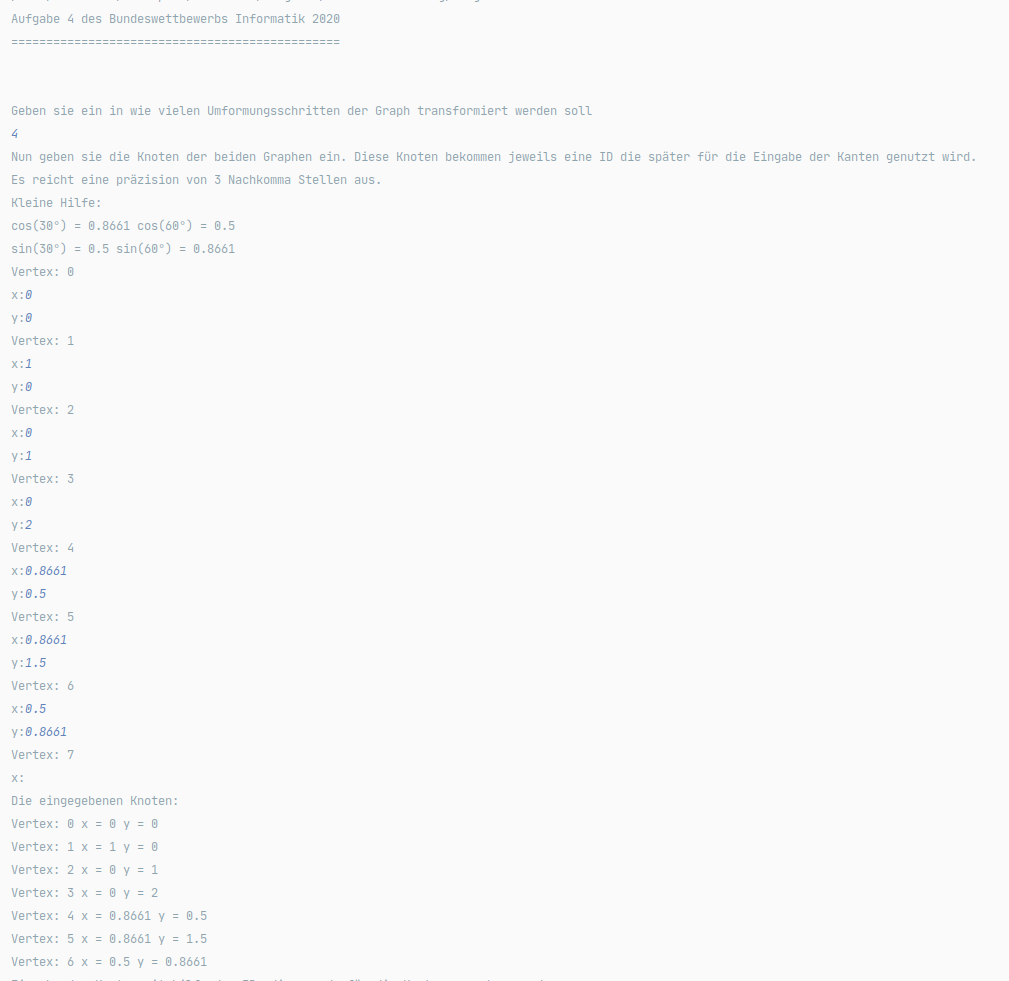
\includegraphics[width=1.05\textwidth]{vertex.png}
	\caption{Selbst erdachtes Beispiel Eingabe der Knoten}
\end{figure}

\begin{figure}[h]
	\center
	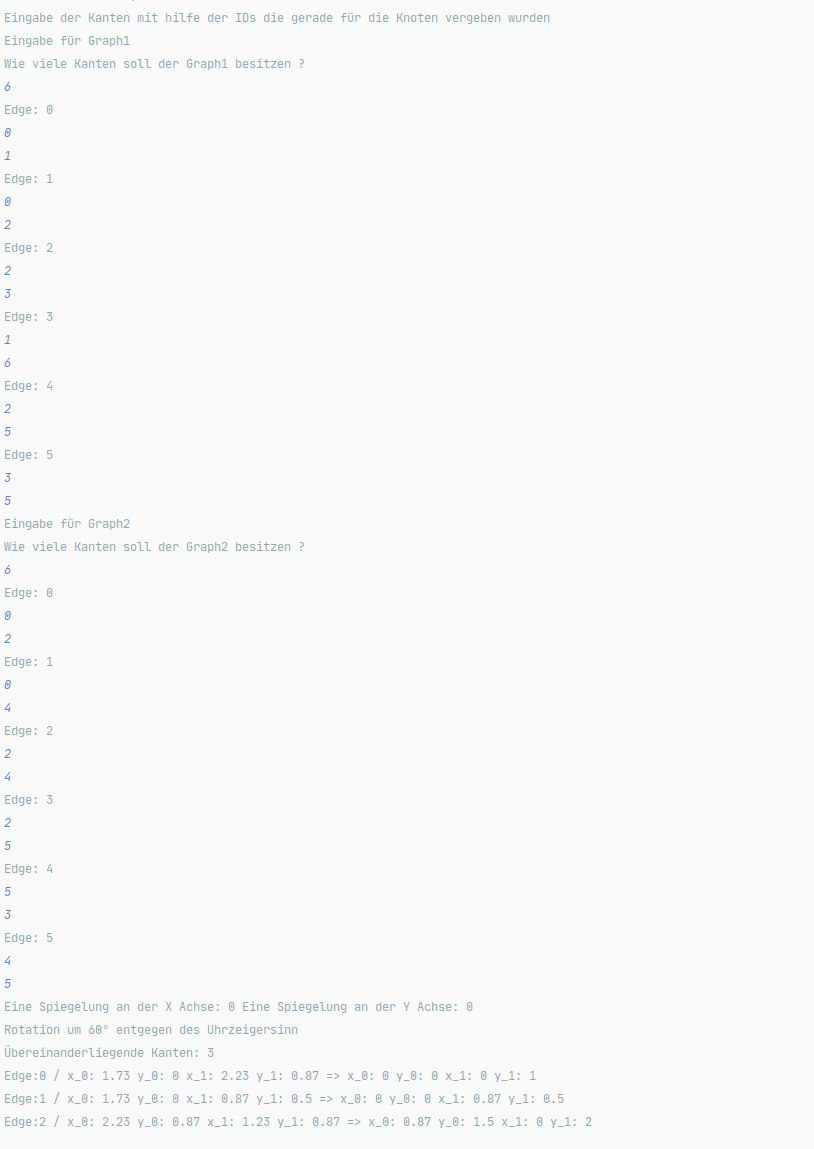
\includegraphics[width=0.8\textwidth]{edge.png}
	\caption{Selbst erdachtes Beispiel Eingabe der Kanten}
\end{figure}

\end{document}
